\section{1174053 - Dini Permata Putri}

\subsection{Teori}
\begin{enumerate}
\item Klasifikasi teks\\
Klasifikasi adalah suatu proses yang memiliki tugas terpenting dalam pemrosesan bahasa alami (natural languange processing), pada proses ini berupa mengklasifikasikan string teks atau dokumen kedalam kategori yang berbeda yang tergantung pada konten string. dalam klasfikasi teksi terdapat berbagai aplikasi seperti mendeteksi sentimen pengguna dari tweet, mengklasifikasikan email sebagai spam, mengklasifikasikan posting blog kedalam kategori yang berbeda, dan sebagainya. contoh dari klasifikasi teks seperti ketika kita akan mencari kata kucing, sedang, makan, ikan lalu jika kata yang dimaksud tersebut sesuai, maka akan menampilkan bilangan biner 1 dan jika salah akan menampilkan bilangan biner 0. seperti yang terlihat pada gambar berikut :
\hfill\break
	\begin{figure}[H]
		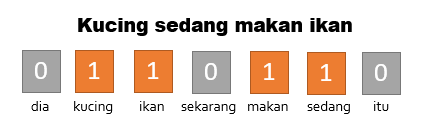
\includegraphics[width=4cm]{figures/1174053/4/1.png}
		\centering
		\caption{Klasifikasi Teks}
	\end{figure}

\item Mengapa Klasifikasi bunga tidak bisa menggunakan machine learning\\
Klasifikasi bunga tidak bisa menggunakan machine learning karena tidak semua bunga memiliki ciri-ciri yang sama, dalam kata lain terdapat data noise dalam klasifikasi bunga sehingga tidak bisa menggunakan machine learning. Contohnya seperti bunga terompet yang memiliki warna merah dengan jumlah kelopak bunga 5. lalu ada bunga warna merah lainnya dengan jumlah kelopak yang sama namun ternyata bukan bunga terompet disamping memiliki kategori yang banyak sekali. bahkan juga terdapat bunga yang tidak jelas dengan warna yang sesuai atau tidak, sehingga bisa menyebabkan data noise.
\hfill\break
	\begin{figure}[H]
		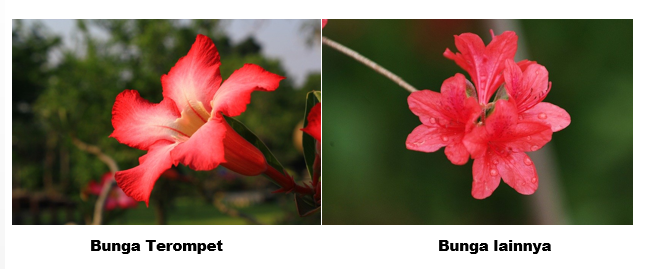
\includegraphics[width=4cm]{figures/1174053/4/2.png}
		\centering
		\caption{Klasifikasi Bunga}
	\end{figure}

\item Teknik pembelajaran mesin pada teks pada kata-kata yang digunakan di youtube\\
Kita ambil sebuah kasus yang semua orang telah ketahui dan juga pahami. Kasus tersebut yaitu perekomendasian video dari pencarian menggunakan ”text / kata” di Youtube. Pada saat menggunakan Youtube terdapat Machine Learning yang bekerja dan memproses perintah ataupun aktivitas tersebut, dimana akan memlter secara otomatis video yang disesuaikan dengan ”keyword” yang kita masukkan sehingga memberikan keluaran video dengan keyword yang benar. Adapula tur yang di dapatkan ketika sedang menonton Youtube. Tampilan sebelah kanan terdapat pilihan ’Next’ atapun ’Suggestion’ yang menampilkan beberapa video serupa sesuai dengan yang dicari atau sedang ditonton. Ketika mengklik salah satu video dari baris tersebut, maka Youtube akan mengingat dan menggunakan kata yang tertera sebagai referensi kembali sehingga akan memberikan kemudahan pada pencarian yang lainnya, Dan disitulah mesin belajar sendiri dan menyimpan data secara berkala sehingga berkembang.
\hfill\break
	\begin{figure}[H]
		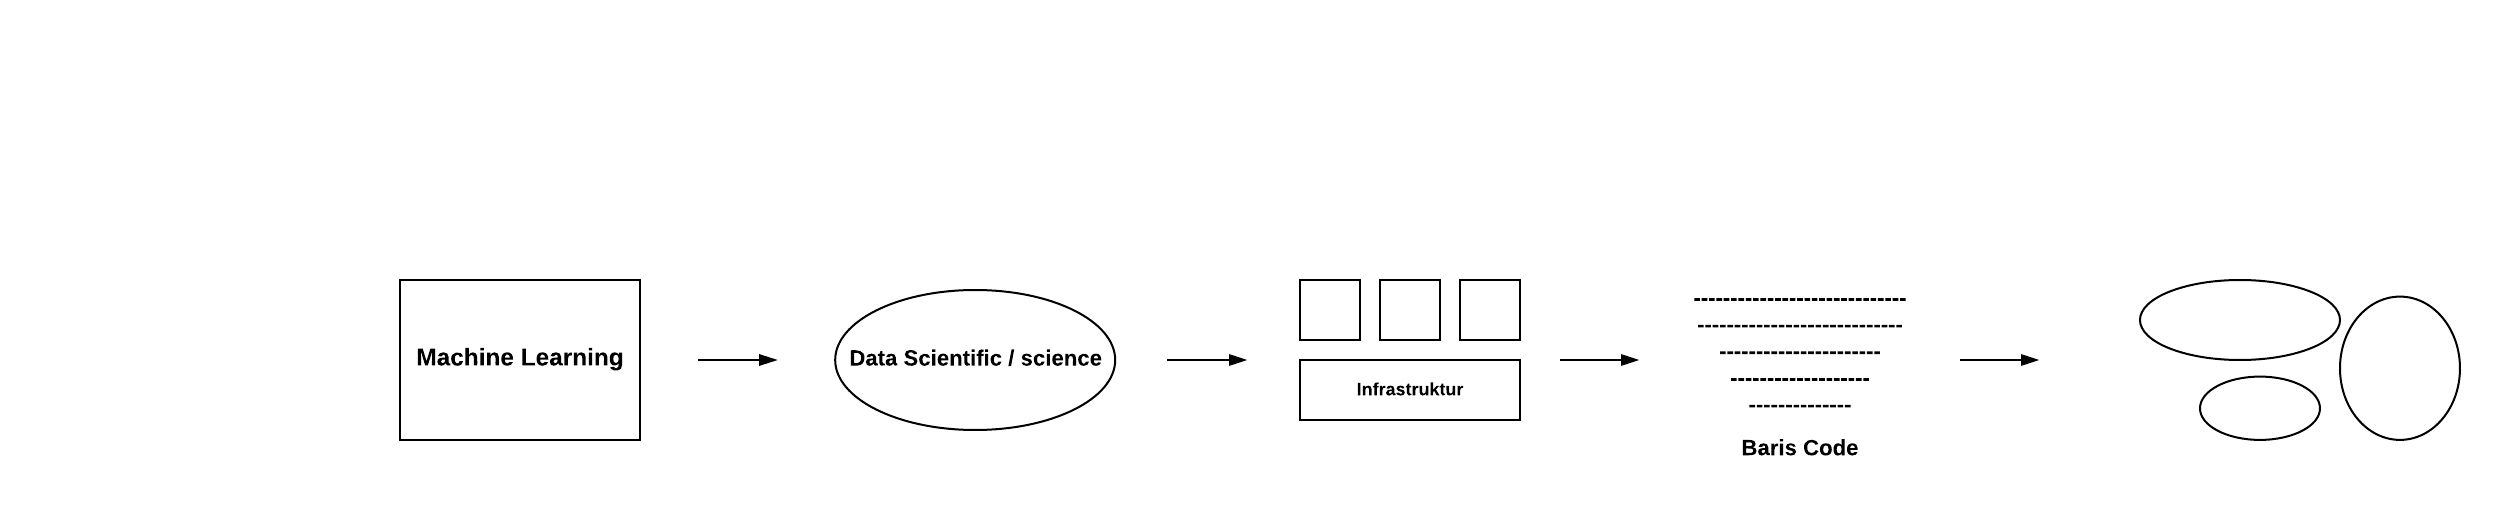
\includegraphics[width=4cm]{figures/1174053/4/3.png}
		\centering
		\caption{Teknik Pembelajaran Mesin}
	\end{figure}

\item Vektorisasi Data\\
Vektorisasi data adalah salah satu proses pembagian dan pemecahan data yang kemudian dilakukan perhitungan. Vektorisasi dapat juga diartikan sebagai setiap data yang mungkin dipetakan ke integer tertentu dan jika memiliki array yang cukup besar maka setiap kata atau data yang cocok dengan slot unik dalam array. 

\item Bag Of Words\\
Bag of words adalah sebuah gambaran yang sederhana yang digunakan untuk pengolahan bahasa alami dan juga pencarian suatu informasi, yang juga dikenal sebagai model ruang vektor, pada model ini tiap kalimat dalam dokumen digambarkan sebagai token kemudian mengabaikan tata bahasa bahkan urutan kata tapi mampu menghitung frekuensi kejadian atau kemunculan kata dari dokumen.
\hfill\break
	\begin{figure}[H]
		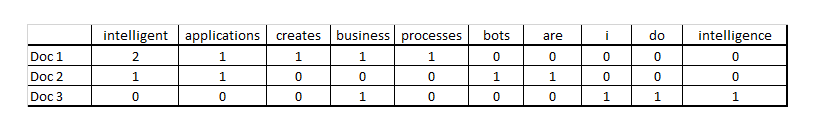
\includegraphics[width=4cm]{figures/1174053/4/4.png}
		\centering
		\caption{Bag Of Words}
	\end{figure}

\item TF-IDF\\
TF-IDF merupakan proses atau tahap yang memberikan frekuensi kata dalam setiap dokumen dalam korpus atau mengganti data menjadi number. Hal ini berupa rasio yang berapa kali muncul dalam dokumen dibandingkan dengan jumlah total kata dalam dokumen. hal ini meringkat seiring jumlah kemunculan kata didalam dokumen juga meningkat. setiap dokumen memiliki tf sendiri. berikut contoh TF-IDF :
\hfill\break
	\begin{figure}[H]
		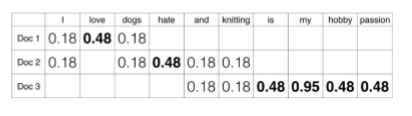
\includegraphics[width=4cm]{figures/1174053/4/5.png}
		\centering
		\caption{TF-IDF}
	\end{figure}

\end{enumerate}

\subsection{Praktek}
\begin{enumerate}
\item Nomor 1
\lstinputlisting[firstline=12, lastline=14]{src/1174053/4/1174054.py}
Hasilnya :
\hfill\break
	\begin{figure}[H]
		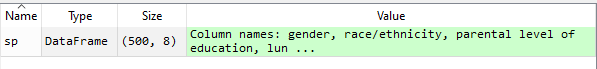
\includegraphics[width=4cm]{figures/1174053/4/6.png}
		\centering
		\caption{Hasil Nomor 1}
	\end{figure}
	
\item Nomor 2
\hfill\break
	\lstinputlisting[firstline=17, lastline=18]{src/1174053/4/1174053.py}
Hasilnya :
\hfill\break
	\begin{figure}[H]
		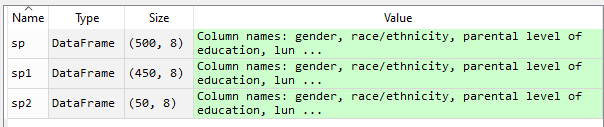
\includegraphics[width=4cm]{figures/1174053/4/7.png}
		\centering
		\caption{Hasil Nomor 2}
	\end{figure}
	
\item Nomor 3
\hfill\break
	\lstinputlisting[firstline=22, lastline=45]{src/1174053/4/1174054.py}
Hasilnya :
\hfill\break
	\begin{figure}[H]
		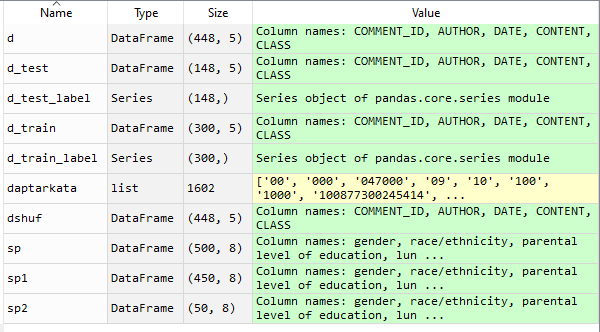
\includegraphics[width=4cm]{figures/1174053/4/8.png}
		\centering
		\caption{Hasil Nomor 3}
	\end{figure}
	
\item Nomor 4
\hfill\break
	\lstinputlisting[firstline=56, lastline=59]{src/1174053/4/1174053.py}
Hasilnya :
\hfill\break
	\begin{figure}[H]
		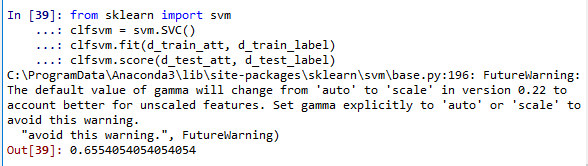
\includegraphics[width=4cm]{figures/1174053/4/9.png}
		\centering
		\caption{Hasil Nomor 4}
	\end{figure}	

\item Nomor 5
\hfill\break
	\lstinputlisting[firstline=49, lastline=52]{src/1174053/4/1174054.py}
Hasilnya :
\hfill\break
	\begin{figure}[H]
		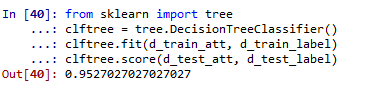
\includegraphics[width=4cm]{figures/1174053/4/10.png}
		\centering
		\caption{Hasil Nomor 5}
	\end{figure}
	
\item Nomor 6\\
Plot Confusion Matrix dari Decision Tree
	\begin{figure}[H]
		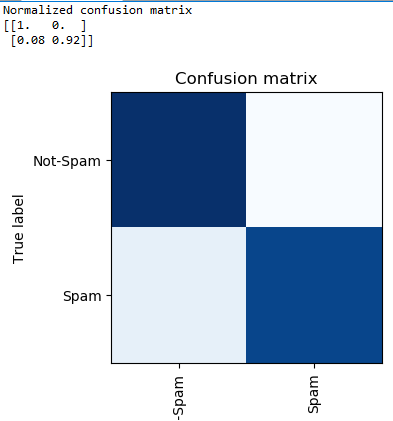
\includegraphics[width=4cm]{figures/1174053/4/11.png}
		\centering
		\caption{Hasil Nomor 6-1}
	\end{figure}
	
Plot Confusion Matrix dari SVM
\begin{figure}[H]
		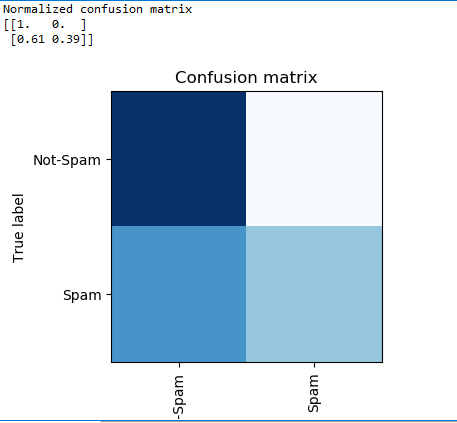
\includegraphics[width=4cm]{figures/1174053/4/12.png}
		\centering
		\caption{Hasil Nomor 6-2}
	\end{figure}
	
\item Nomor 7
\hfill\break
	\lstinputlisting[firstline=169, lastline=178]{src/1174053/4/1174053.py}
Hasilnya :
\hfill\break
	\begin{figure}[H]
		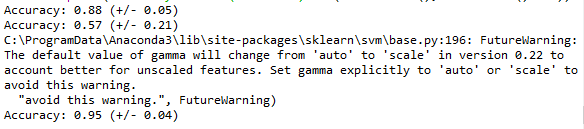
\includegraphics[width=4cm]{figures/1174053/4/13.png}
		\centering
		\caption{Hasil Nomor 7}
	\end{figure}
	
\item Nomor 8
\hfill\break
	\lstinputlisting[firstline=182, lastline=195]{src/1174053/4/1174053.py}
Hasilnya :
\hfill\break
	\begin{figure}[H]
		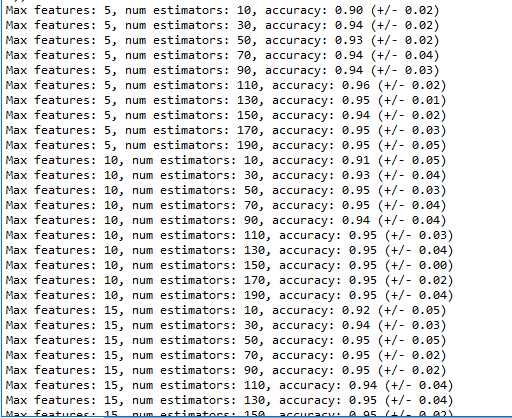
\includegraphics[width=4cm]{figures/1174053/4/14.png}
		\centering
		\caption{Hasil Nomor 8}
	\end{figure}
\end{enumerate}

\subsection{Penanganan Error}
\begin{enumerate}
\item ScreenShoot Error
	\begin{figure}[H]
		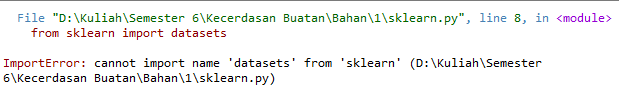
\includegraphics[width=4cm]{figures/1174053/4/error.png}
		\centering
		\caption{File Not Found Error}
	\end{figure}

	\item Tuliskan Kode Error dan Jenis Error
	\begin{itemize}
		\item File Not Found Error

	\end{itemize}
	\item Cara Penanganan Error
	\begin{itemize}
		\item File Not Found Error
		\hfill\break
		Error terdapat pada kesalahan baca file csv, yang tidak terbaca. Dikarenakan letak file yang dibaca tidak para direktori yang sama. Seharusnya letakkan file di direktori yang sama. 
	\end{itemize}
\end{enumerate}


\subsection{Bukti Tidak Plagiat}
\begin{figure}[H]
	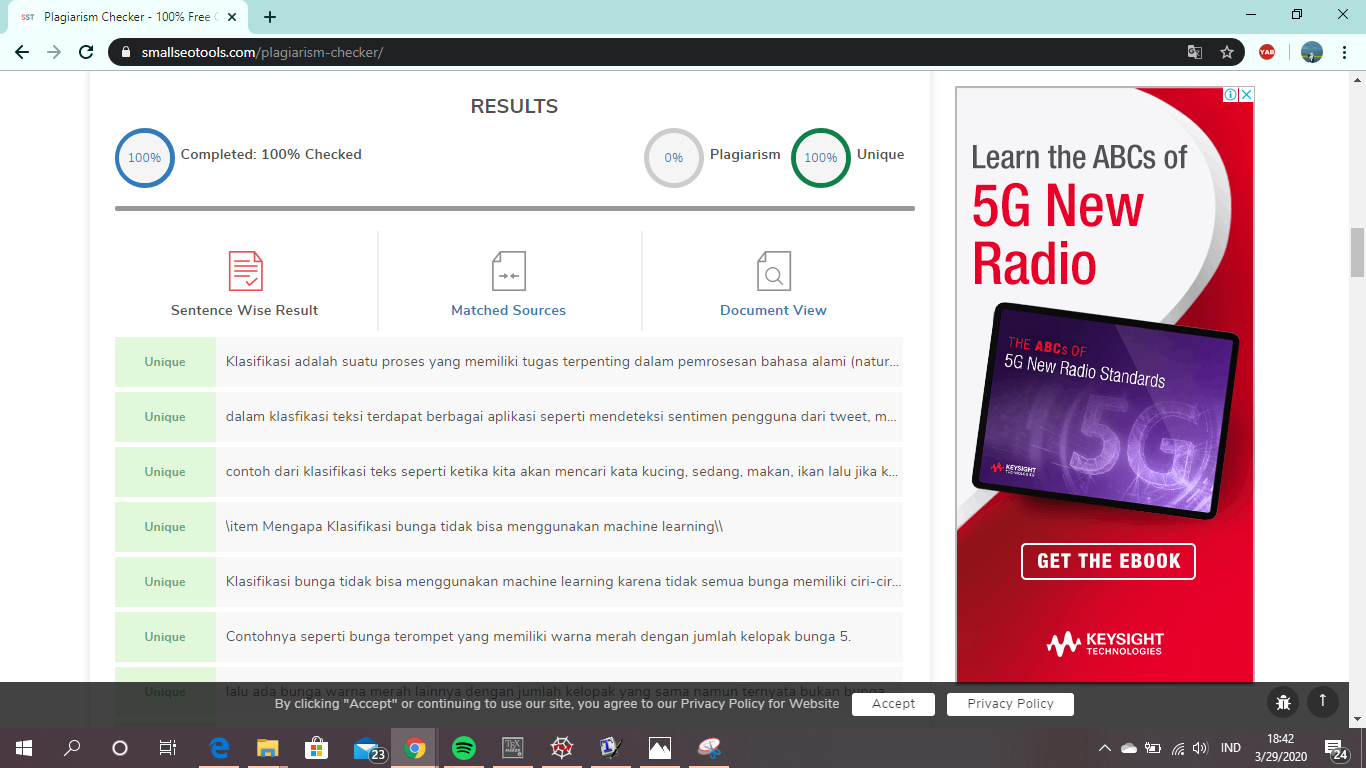
\includegraphics[width=4cm]{figures/1174053/4/plagiarisme.png}
	\centering
	\caption{Bukti Plagiasrisme}
\end{figure}

\subsection{Link Youtube}
